\chapter{Introduction and Background}
\label{ch: intro}

\graphicspath{{Figures/Intro/}{./}} 

\section{Quantiles}
\label{sec: intro_quant}
Quantiles are the cutting points of a statistical distribution by its ranking. Specifically, the $\tau$-quantile is the cutting point that divides the distribution by probability $\tau$. Let $\tau$-q denotes the $\tau$-quantile. For example, a $0.5$-q is the median of a distribution, such that there is a $50\%$ probability that a random sample is smaller than it. Generally, the value of a quantile can be achieved by mathematical approaches when the expression of the distribution is given. 
The quantiles are an important statistical feature of distributions for their values roughly reflects the density of the distribution.
For example, Fig \ref{fig: quant_example} shows the two intervals of the sampling from a Gaussian distribution between [$0.5$-q, $0.9$-q] and [$0.9$-q, $0.99$-q] has similar value, while the former contains 40\% data and the latter contains only 9\% data. Without any other information, this alone leads to the implication that the distribution is denser in the former interval than the latter.

\begin{figure*}[h!]
    \centering
	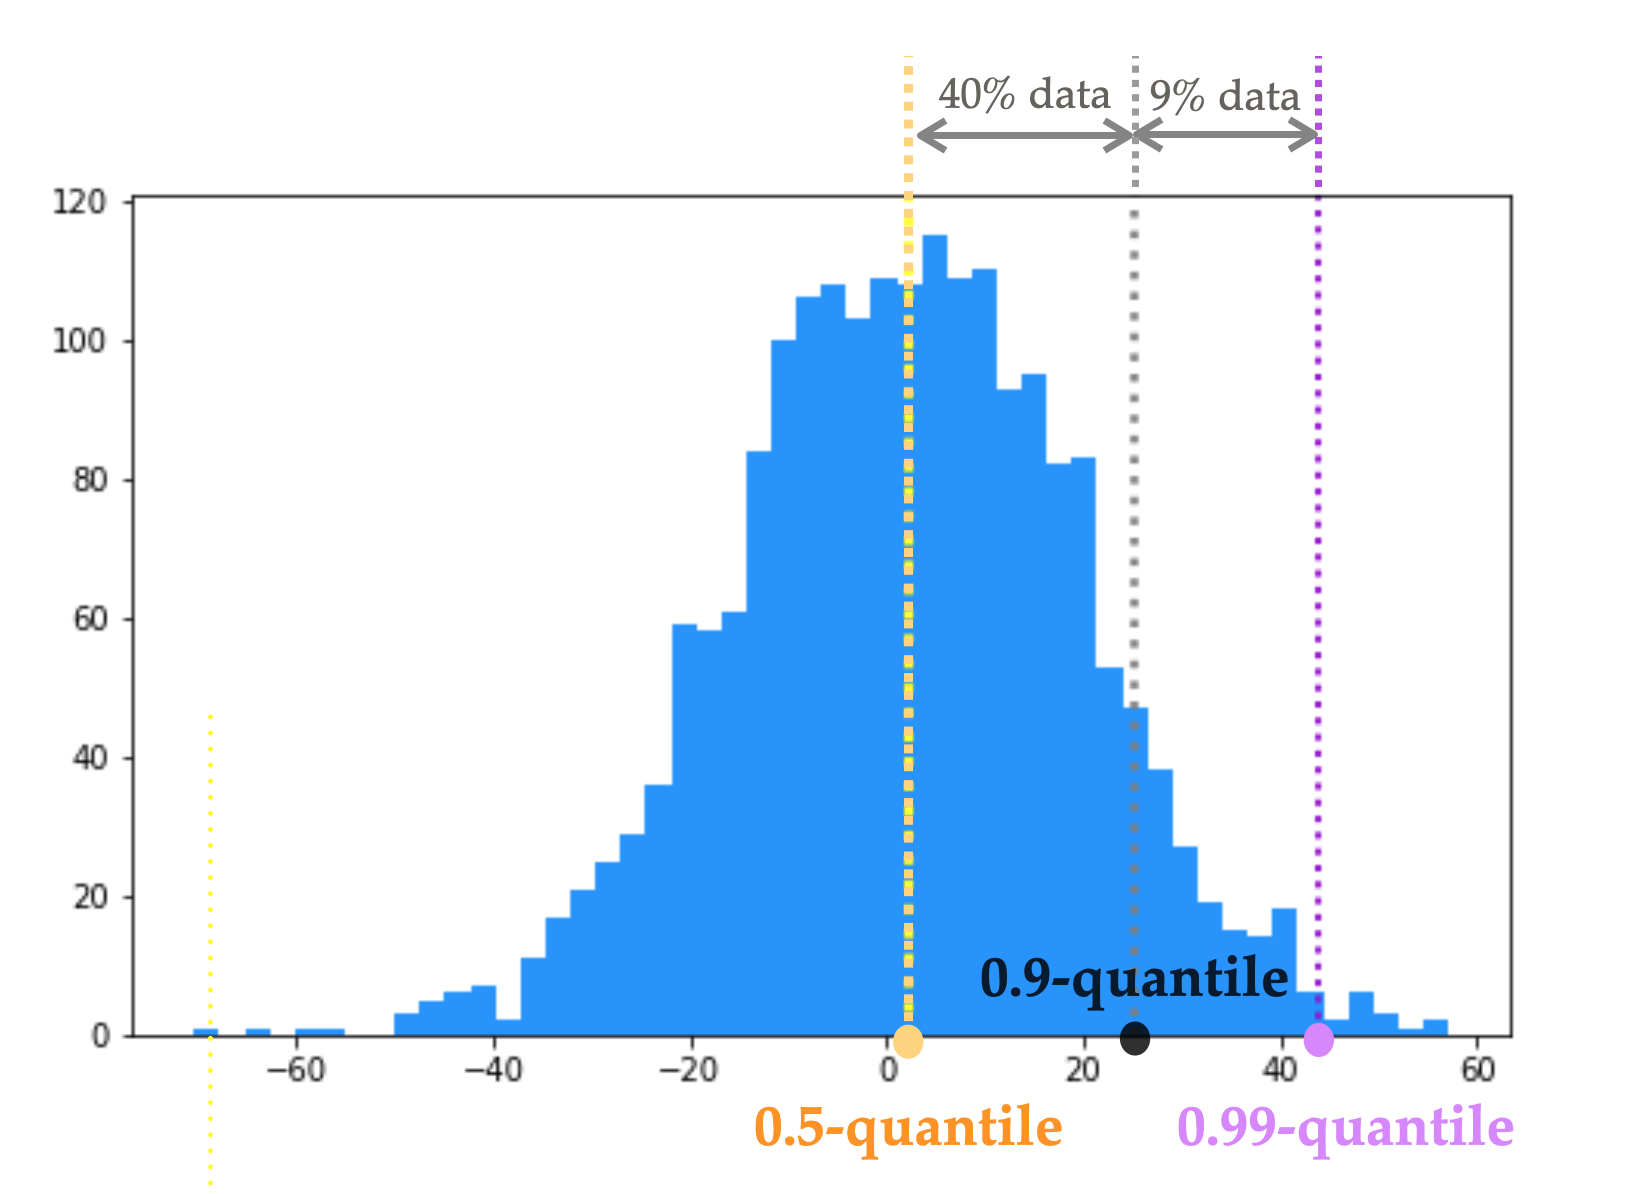
\includegraphics[width=0.6\columnwidth]{quant_example.png}
    \caption{Quantiles (0.5-q, 0.9-q and 0.99-q) of a dataset containing 2000 random samples from a Gaussian distribution (mean = 2, standard deviation = 18)}
    \label{fig: quant_example}
\end{figure*}

As shown in the example of Fig \ref{fig: quant_example}, the concept of quantiles are also applied in datasets besides probability distributions. Similarly, the quantile for a finite dataset is also the point which divides the dataset by probability $\tau$. However, since the dataset is discrete, the value of a $\tau$-q is ambiguous. E.g. for dataset [$1,2,3,4$], both 2.01 and 2.99 can be considered as a valid value of $0.5$-q. Among various methods of dataset quantile estimations, we apply the one currently used by the \textit{Python 3} language. For a size $N$ dataset $X = \{x_1, ..., x_N\}$ , the method first finds the ranking index of the quantile $h = (N-1)\tau + 1$. If $h$ is not an integer, the estimated quantile is computed by linear interpolation between the two data points at ranking positions surround $h$
\begin{equation}
    \tau \text{-q}_{batch} = x_{\lfloor h\rfloor}+(h-\lfloor h\rfloor)\left(x_{\lfloor h\rfloor+1}-x_{\lfloor h\rfloor}\right)
\end{equation}
where $\lfloor h\rfloor$ is the greatest integer less than or equal to $h$. The computation result $\tau \text{-q}_{batch}$ is called a \textit{batch quantile}, since it comes from a batch of samples of a distribution.
\\\\
Note although the computation of batch quantiles are estimation of quantiles of a distribution sample, it is \textit{not} what is referred to as "quantile estimation" in this paper. Here the batch quantiles are regarded as computed quantiles, as a comparison of \textit{true quantiles} which are the real quantiles of the original probability distribution. The estimation of quantile is introduced in the following part.

% Batch algorithm/True quantile: the naive sorting

\section{Data streams and quantile estimation}
\label{sec: intro_quant_est}

\textit{Data streams} is the phenomenon when a large amount of data come in sequence of a stream-like form. To distinguish from datasets, data points are not instantly available all at a time, and that the size of the sample keeps growing. It is commonly seen in areas like network monitoring, data mining, financial trading systems, etc. Similar to normal dataset, the value of quantiles is also important for data analysis on data streams. Finding the quantiles of a data stream is the motivation of this paper.

A trivial solution to find quantiles of data streams is to sort the entire data stream when the last data point arrives, and then compute the batch quantiles of the sorted dataset.  In cases when the size of the data stream is unknown, at the arrival of each data point, the batch quantiles are computed again so the quantile values get updated. The method of repeatedly sorting and compute batch quantiles is called the \textit{batch algorithm}. Due to the large size of the data streams, the batch algorithm for quantile computation is too expensive in both storage and computation to be a feasible solution for most computer systems.
\\\\
Faced with the storage and computation problem, algorithms of \textit{quantile estimation} on data streams have been proposed. The quantile estimation algorithms do not store the entire data streams, and the algorithms return estimated quantile that are close to the batch quantiles. Some of the algorithms are gone through in the literature review chapter. Although the storage has been reduced by a significant amount, most algorithms still require a growing space complexity (e.g. correlated with size $N$). This paper is especially interested in the space-efficient algorithms that uses constant memory units for data streams of any size. Specifically, we focus on the machine learning method \textit{stochastic gradient descent} (SGD) for quantile estimation. 

\section{Stochastic gradient descent(SGD) for quantile estimation}
\label{sec: intro_GD_SGD}

\textit{Gradient descent} is a convex optimization algorithm that is commonly used in machine learning for loss function minimization. The gradient descent takes the entire dataset as the input, and by iteratively moving in the opposite direction of the gradient descent, it reaches the targeting results of local minimum. Such method can also be used in quantile estimation if the entire dataset is available all at the same time.

\textit{Stochastic gradient descent (SGD)}, on the other hand, is the "online learning" version of gradient descent that updates the optimization iteratively when every new data point comes. Each step is moved in the opposite direction of the gradient computed from the coming data point, which uses a subset of data to replace the whole dataset. Fig \ref{fig: SGD_quant} shows how SGD is used to estimate quantiles on the same dataset of 2000 Gaussian distribution samples. It is shown in the figure that the SGD result fluctuates around the empirical quantile value, indicating SGD is a possible approach for quantile estimation.

\begin{figure*}[h!]
    % \centering
	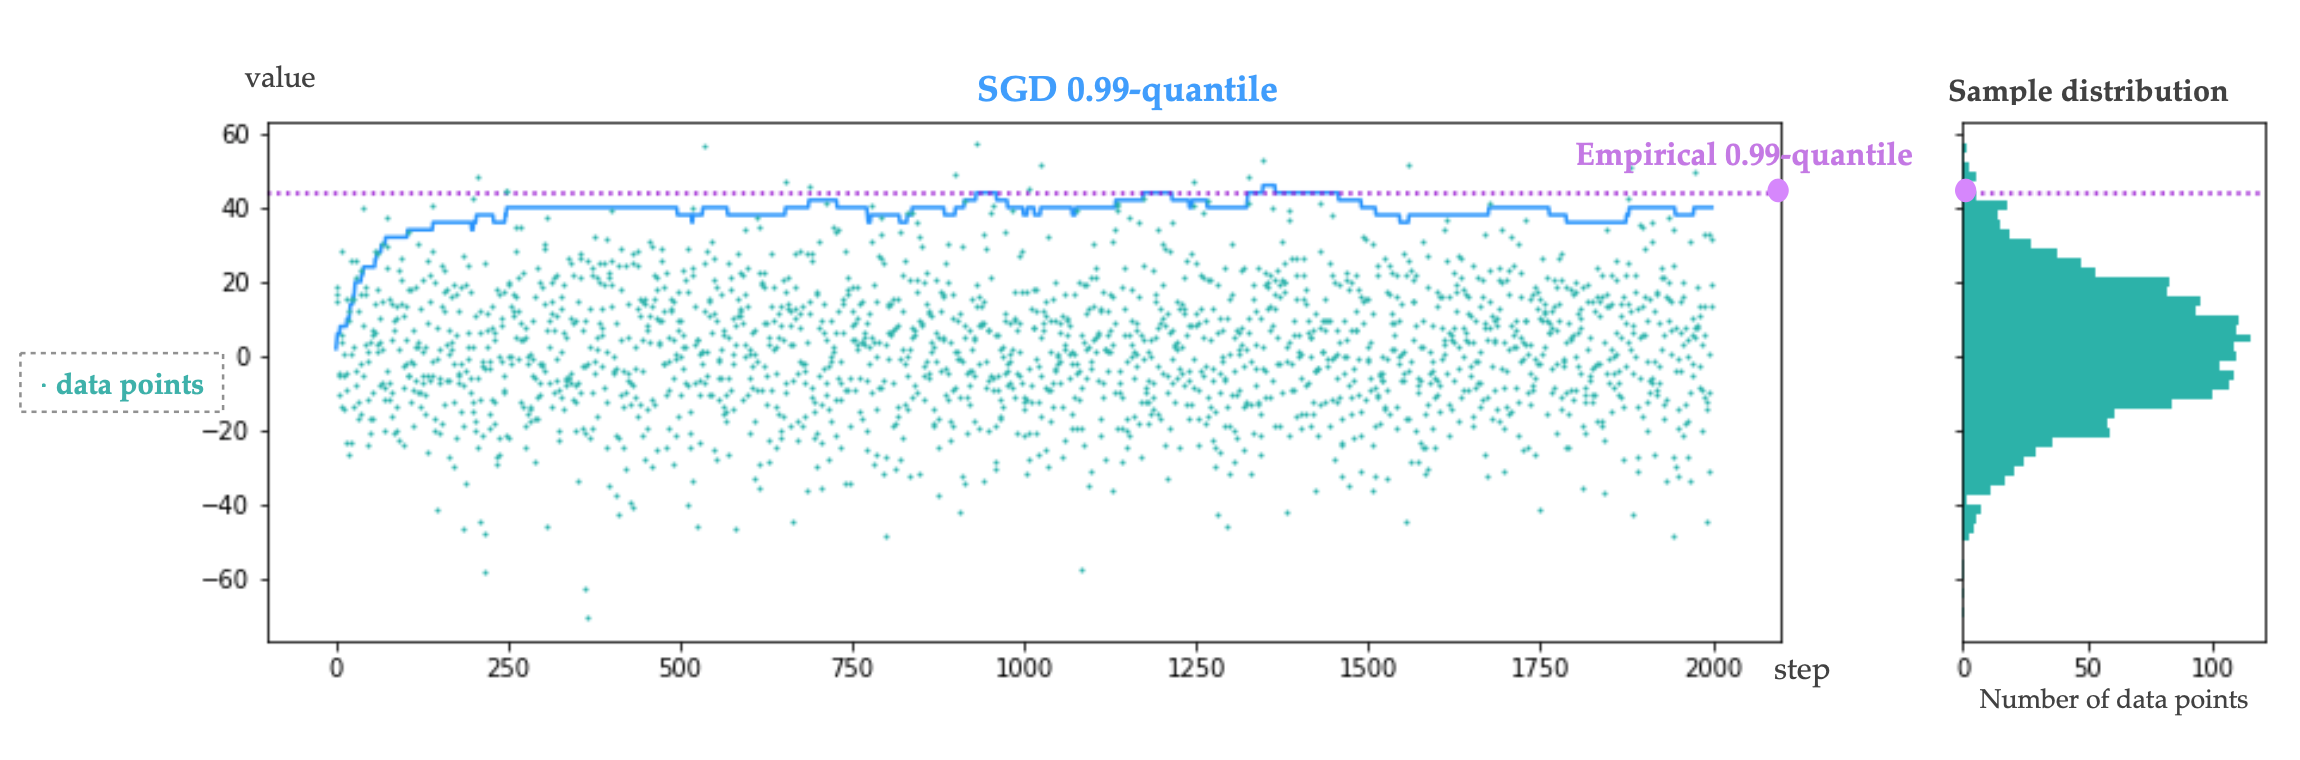
\includegraphics[width=1\columnwidth]{SGD_gaussian.png}
    \caption{SGD quantile estimation of the $0.99$-q for a dataset of 2000 samples from a Gaussian distribution. The left graph is a combination of incoming data points and the SGD steps, and each step of SGD is triggered by a new coming data point. The blue line shows how the SGD result is updated on the arrival of a data point (sea-green), and straight line (violet) represents the empirical value of $0.99$-q. On the right side, the density of the bell-shaped dataset is shown in a histogram.}
    \label{fig: SGD_quant}
\end{figure*}

\section{Thesis overview}
\label{sec: intro_overview}
In the final part of the introduction, we give a brief tour of the material in this paper.
The main focus of the paper is to explore how stochastic gradient descent method can be used for quantile estimation on data streams.
In chapter \ref{ch: literature_review}, a very brief development of quantile estimation algorithms are introduced, with a special mentioning on space-efficient algorithms (e.g. SGD-like methods). 
Chapter \ref{ch: sgd_equivalence} compares the SGD methods with the \textit{Frugal1U} algorithm\cite{maFrugalStreamingEstimating2014}, showing how the two similar methods are "equivalent" to some extent.
It is followed by chapter \ref{ch: sgd_experiment} where the experiments illustrate relationship between different settings of SGD and the performances. 
Next, chapter \ref{ch: stepsize} and \ref{ch: multi_quant} explore the two extensions of the vanilla SGD algorithm: the step size adaptation of SGD and the simultaneous multi-quantile estimation. Finally, the work of the paper is summed up in the conclusion chapter \ref{ch: conclusion}.
\\\\
Fig \ref{fig: structure} is the layout of the contents of the paper.

\begin{figure*}[h!]
    \centering
	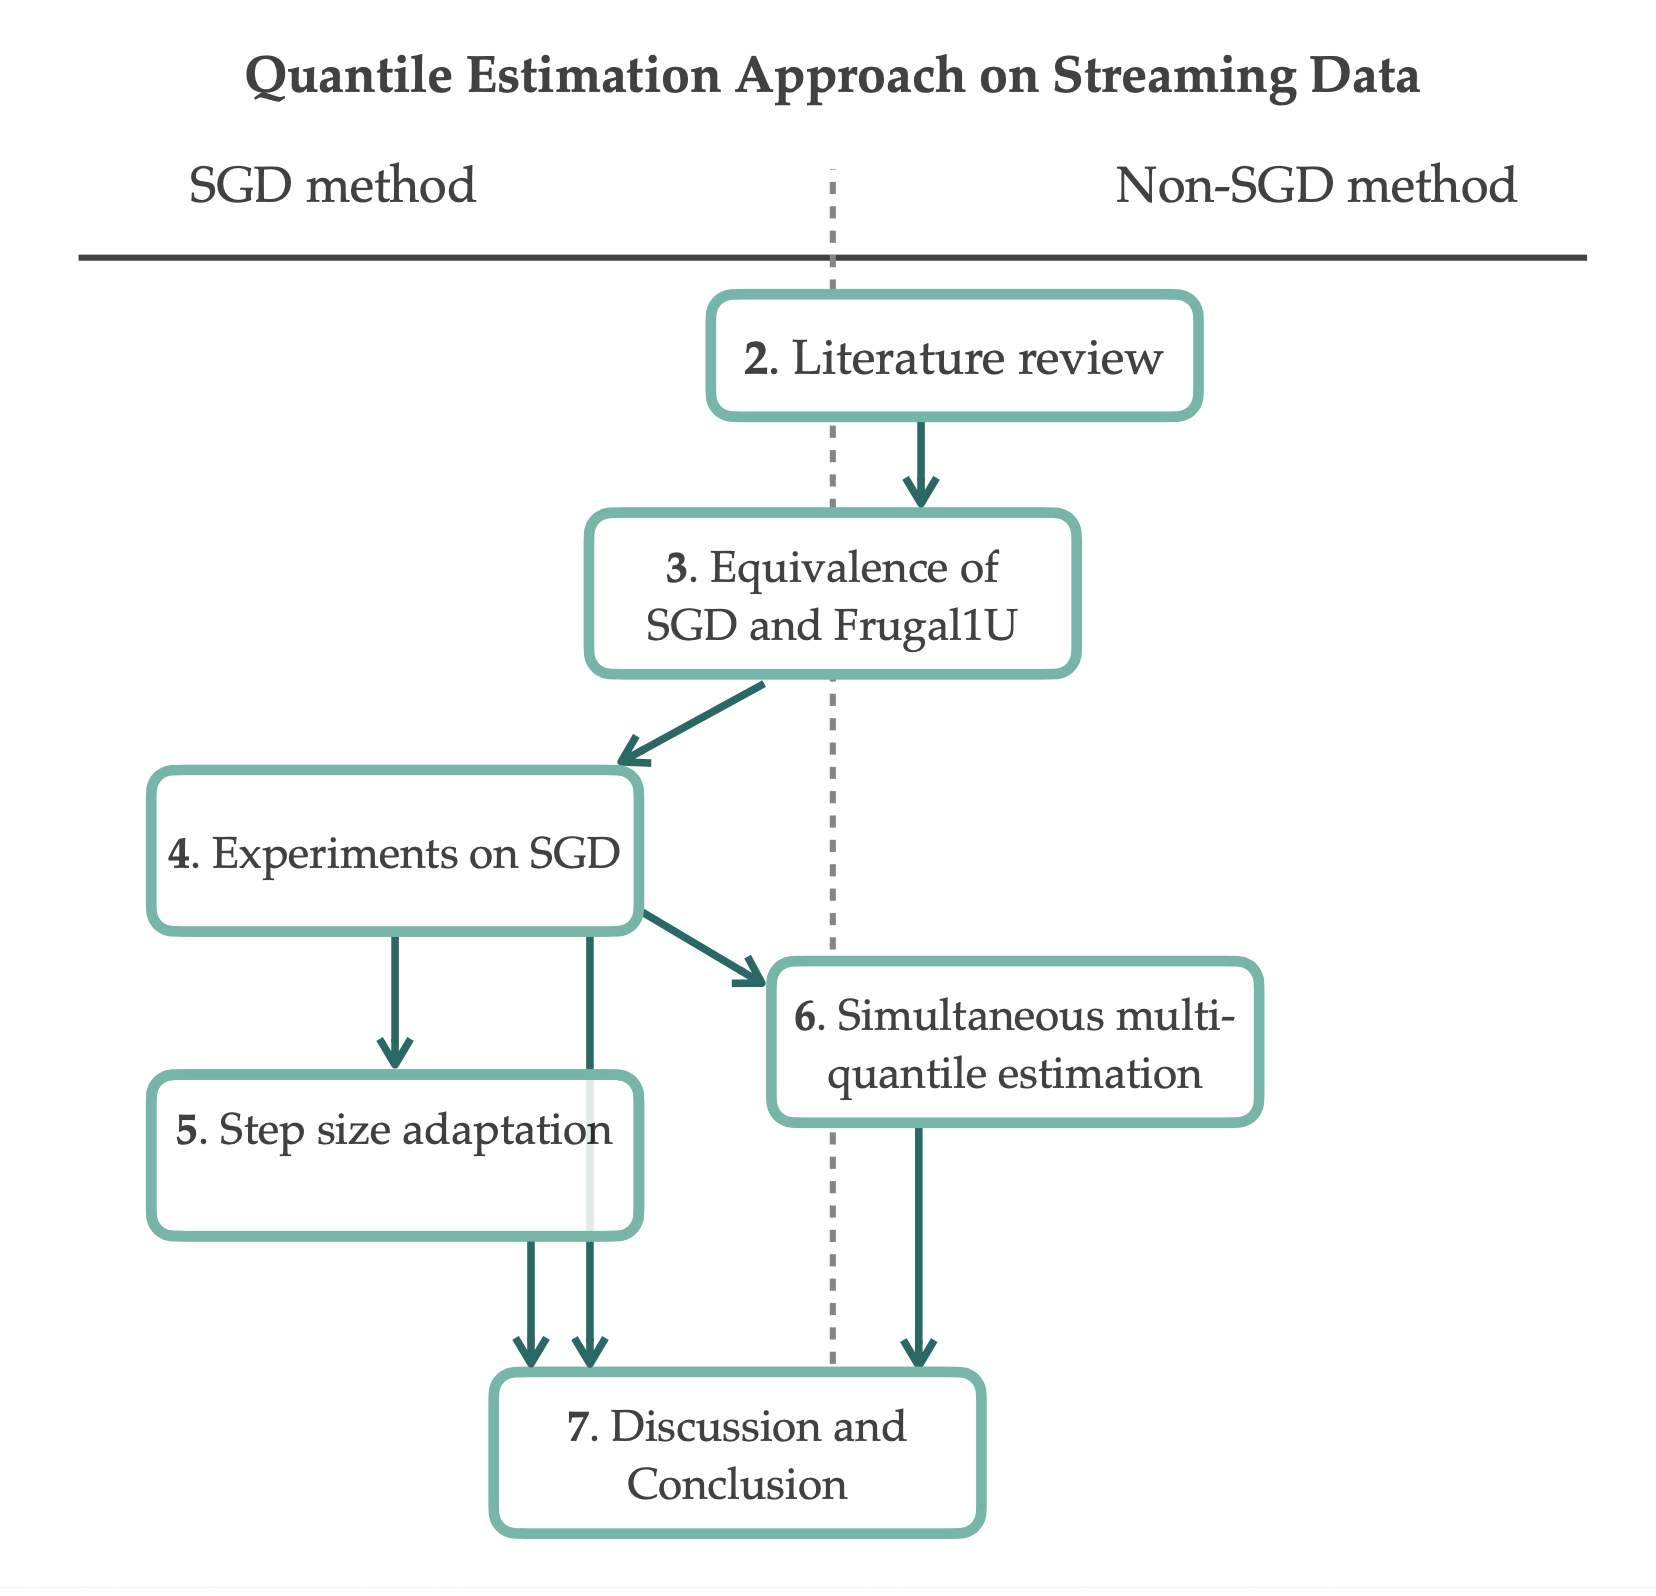
\includegraphics[width=0.8\columnwidth]{structure.png}
    \caption{The relationship between topics covered in the thesis. Topics are roughly positioned along the top-bottom axis depending on where they are more close to SGD methods (left) or non-SGD methods (right). The arrows between the chapters represent are connected according to dependence.}
    \label{fig: structure}
\end{figure*}